\subsection{Outgassing of Tritiated Methane from Plastics}
\label{sec:appendix}

\newcommand*{\Scale}[2][4]{\scalebox{#1}{$#2$}}%

An accurate model of a tritiated methane injection into LUX must account for outgassing of CH$_3$T from plastics such as polyethylene and teflon. Duhamel's priciple, an integral solution to Fick's second law on a half-infinite line is found to be
\[\Scale[0.85]{\phi (x,t) = KC_{out} - \int \limits_0^t erf(\frac{x}{\sqrt{4D(t - \tau)}})K\dot{C_{out}}(\tau)d\tau - KC_{out}(0)erf(\frac{x}{\sqrt{4Dt}}),}\]
where $K$ is the solubility of the material, $D$ is the diffusion constant, and $C_{out}$ is the concentration at the surface of the material. 
%\cite{Piche}
For the outgassing process we are only able to detect the flux of material out of the plastic.  This is given by Fick's first law evaluated at $x=0$,
\[J_{out}(t)= - K \sqrt{\frac{D}{\pi}}\left( \int \limits_0^t \frac{\dot{C_{out}}(\tau)}{\sqrt{t-\tau}} d \tau + \frac{C_{out}(0)}{\sqrt{t}}\right),\]
where the sign has been flipped since the flux of material is outward.  It is no longer possible to evaluate $K$ and $D$ separately, since the diffusion in and out of the plastic is completely determined by the time-dependent concentration outside of the plastic.  To simplify our model, we define a new constant
\[ G = K \sqrt{ \frac{D}{ \pi }} .\] Using data from the LUX sampling system we set an upper limit of $G<0.0016 \frac{cm}{\sqrt{day}}$. 

\begin{figure}[h!]\centering
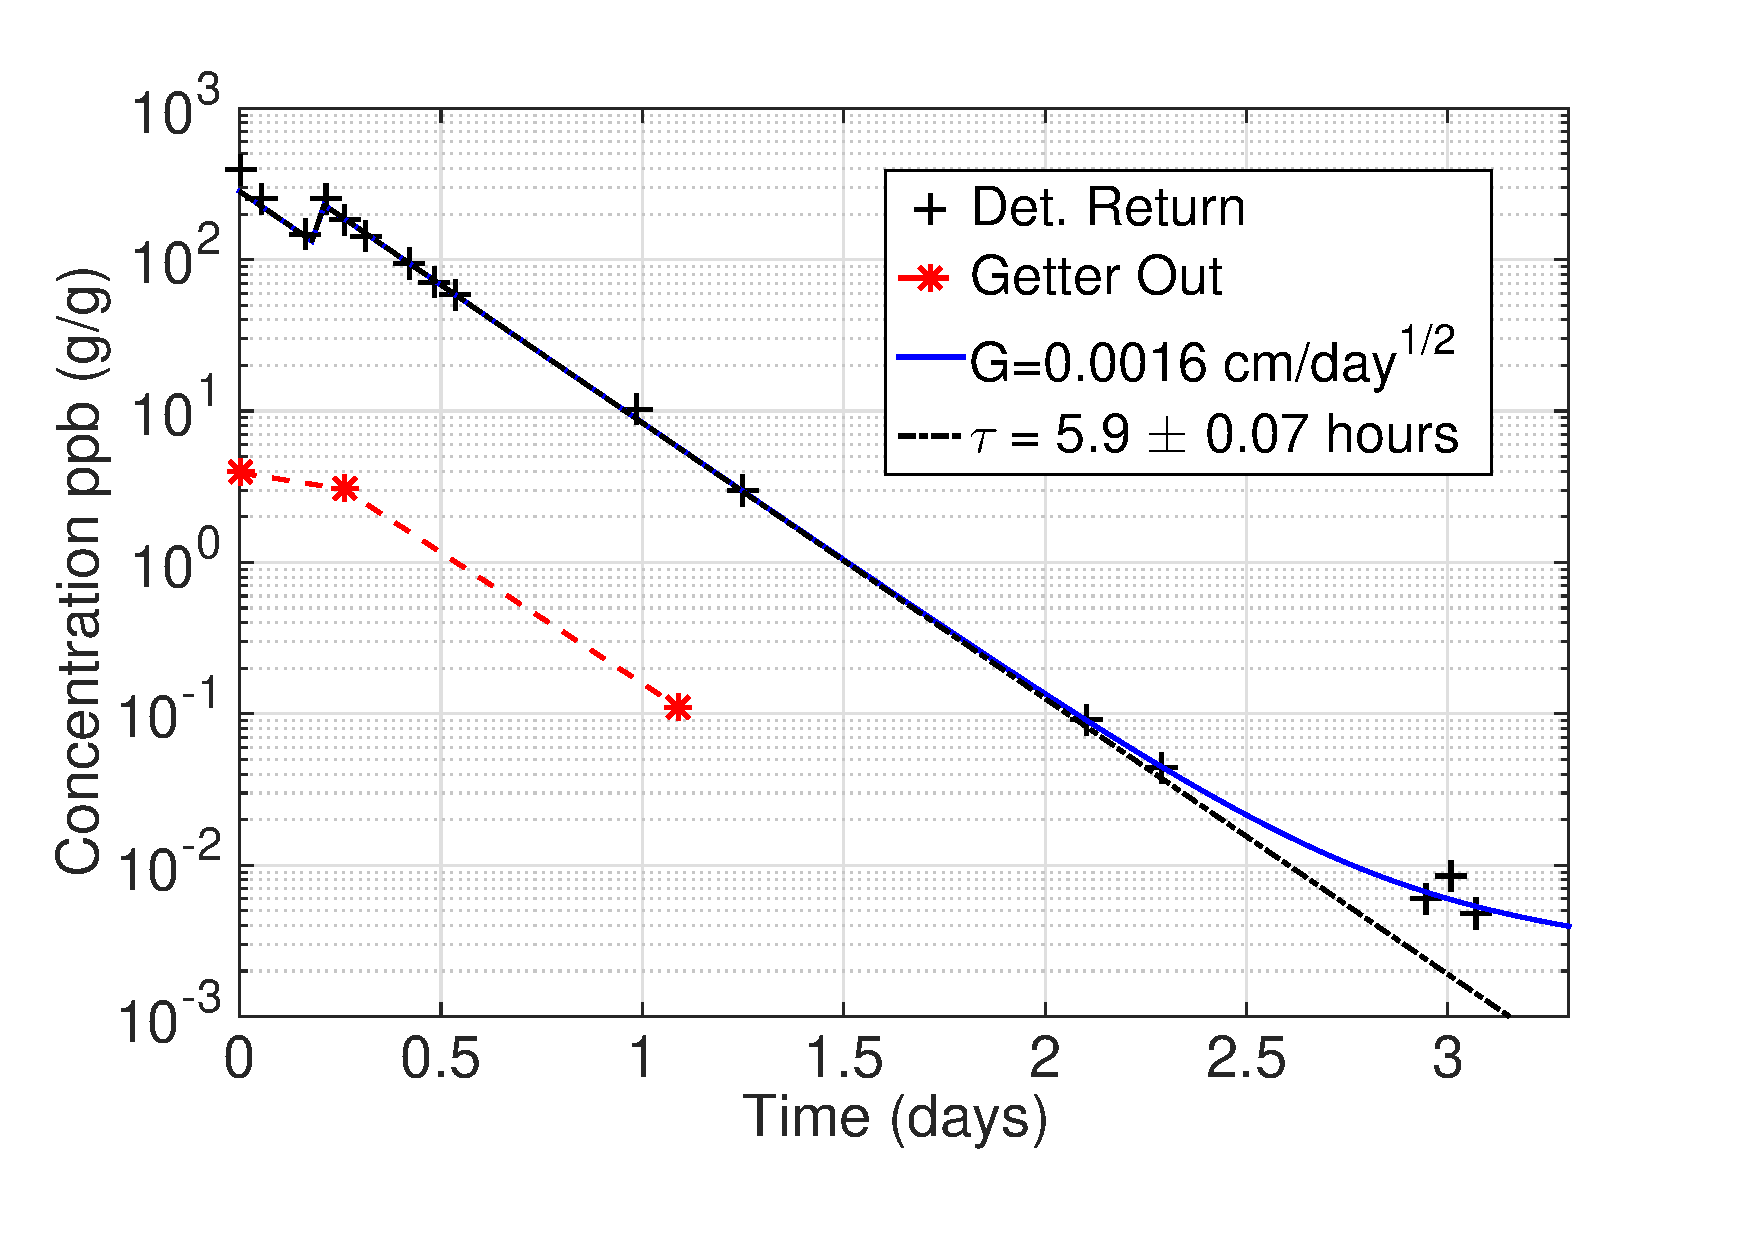
\includegraphics[width=80mm]{fig/July_CH4_wOG.eps}
\caption{Removal of natural methane observed by the integrated xenon sampling system prior to the tritiated methane injections. The red points indicate measurements at the getter outlet, we find a 97\% one pass removal efficiency at a flow rate of 27 SLPM. The blue curve shows the upper limit on the effect of outgassing from the plastics. The black dashed lines shows the exponential fit to the natural methane removal from the xenon with a time constant of 5.9 $\pm 0.07$ hours. $\rm 5\times10^{-3}$ ppb (g/g) is the limit of detection for methane.}
\label{fig:ch4_removal}
\end{figure}

With a constraint on $G$ taken from the analytic solution to Fick's second law, we turn to numerical simulation to answer the question of how much initial CH$_3$T activity to inject into LUX to meet our calibration goals. We set a limit of 0.33 $\mu$Bq (5\% of the LUX ER background rate design goal) from residual CH$_3$T activity after an injection.  Several assumptions are made to simplify the numerical model.  First, we approximate the diffusion into plastic as being a one dimensional process.  Since the plastic in LUX can be approximated by a cylindrical shell there is no dependence on the azimuthal or $z$ coordinates.  Since $r$ is large compared to the thickness of the plastic shell, $\frac{\delta^2 \phi}{\delta r^2} \gg \frac{1}{r} \frac {\delta \phi}{\delta r}$, so Fick's laws in a one dimensional approximation become
\[J=-D\frac{\delta \phi}{\delta r}\vec{r}\]
\[\frac{\delta \phi}{\delta t} = D \frac{\delta^2 \phi}{\delta r^2}.\]  We assume the concentration of CH$_3$T in LUX is uniform throughout its volume, since the design of LUX creates currents which stir the liquid xenon.  With perfect mixing the effect of the purifier can be modeled by adding an exponential time dependence of 5.9 $\pm 0.07$ hours to the outer volume. 

We use a simple implementation of the first order Euler method for to produce numerical simulations of the residual activity in LUX after a CH$_3$T injection. The diffusion is simulated by setting the concentration at the boundary of the piece equal to $KC_{out}$, where $C_{out}$ is the concentration of CH$_3$T in the xenon.  This concentration is dependent on time according to
\[\frac{\delta C_{out}}{\delta t} = J_{out} \frac{A_{plastic}}{V_{xenon}}-\frac{C_{out}}{\tau},\]
where $A_{plastic}$ is the surface area of the plastic cylinder, $V_{xenon}$ is the total volume of xenon in the fiducial region, and $\tau$ is the characteristic removal time of methane from LUX.  The first term on the right of this equation models outgassing of CH$_3$T from the plastic cylinder, while the second term models removal of CH$_3$T through purification.  Using the first order Euler method, we arrive at an expression for $C_{out}$ given by
\[C_{j+1}=C_j + \Delta t \left[(J_{1,j}-J_{N_x,j})\frac{A_{plastic}}{V_{xenon}}-\frac{C_j}{\tau}\right].\]
The initial concentration is defined by dividing the desired injection activity by the volume of the fiducial region.  We choose $D = 2.3 \times 10^{-9} \frac {cm^2}{sec}$ so that the half-infinite boundary conditions in our diffusion model is valid, and combine this with our upper limit on $G$ to extract a value for $K$.  We use this model to predict the total number of calibration events as well as the time required to return to \textless 5\% of the nominal background rate for any CH$_3$T injection into LUX.  

\begin{figure}[h!]
\centering
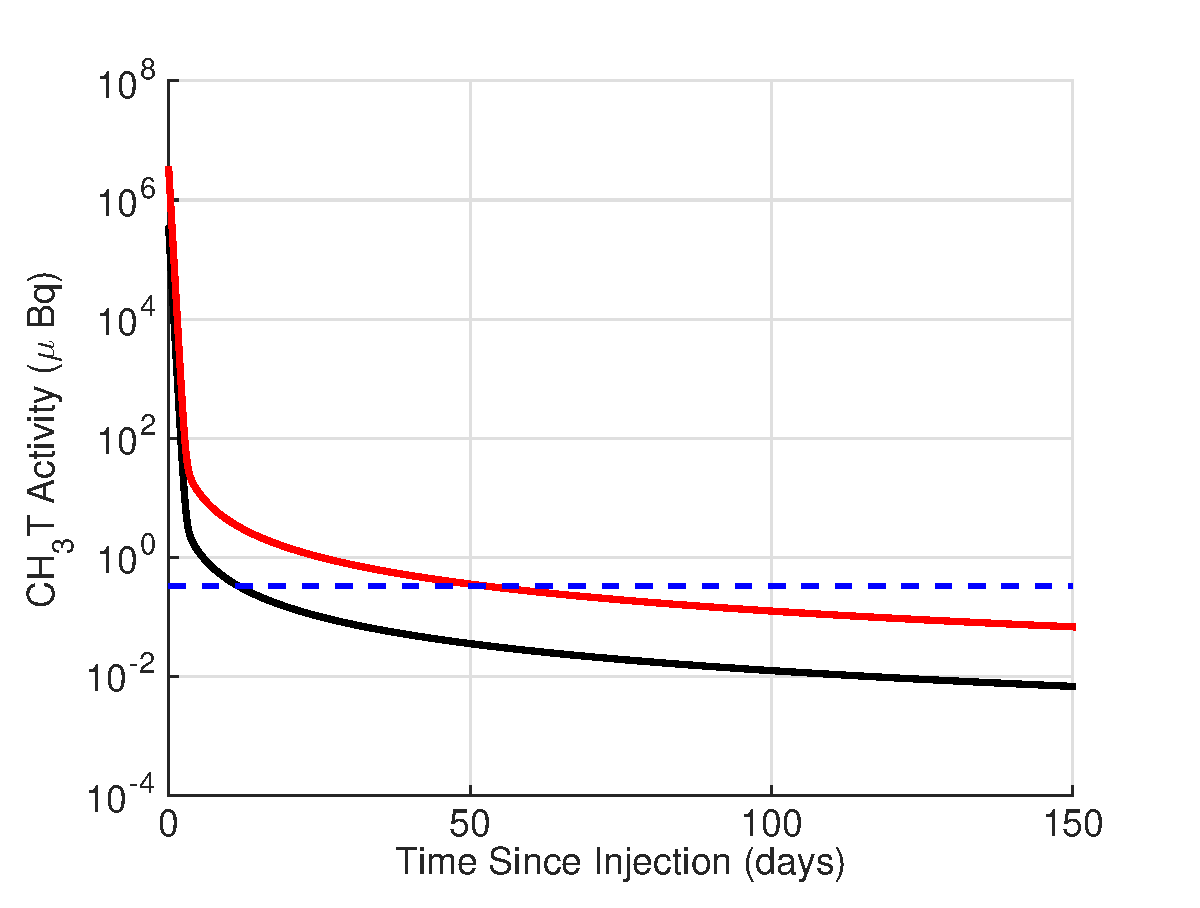
\includegraphics[width=0.95\textwidth]{fig/LUX_og_lim.eps}
\caption{Displayed are the results of simulated outgassing effects from a 1 Bq (black curve) and 10 Bq (red curve) injections of CH$_3$T into LUX. The dashed blue line is the tritium activity goal of 0.33 $\mu$ Bq. The simulated outgassing assumes the upper limit of G taken from the CH$_4$ injection in LUX (0.0016 cm/day$^{1/2}$).}
\label{fig:tau_var}
\end{figure}

Figure \ref{fig:tau_var} shows the results of our simulations for a 1 Bq and 10 Bq injection into LUX.  We find that for moderate injections on the order of 1 Bq we reach our limit of 0.33 $\mu$Bq 8 days after the initial injection.  For larger injections it can take longer than 35 days to reach our background limit.  While these simulations use a conservative upper limit for the value of $G$ it emphasizes that injecting too much CH$_3$T into LUX can lead significant delays in a WIMP search.  


\subsection{Tritiated Methane Removal}
\label{sec:RD}

The removal efficiency of zirconium getters for CH4 in xenon had previously been studied at the University of Maryland.  It was found that greater than 99.99\% of natural methane can be removed in a single pass through a zirconium getter. \cite{Dobi_CH4} Tritiated methane is chemically identical to natural methane, so it follows that similar removal efficiencies should be expected for CH$_3$T.  To verify this a small scale tritiated methane injection system was integrated into a liquid xenon system at the University of Maryland.  This system used a SAES MC1-905F methane purifier placed in series immediately after the CH$_3$T source bottle to prevent non-methane species of tritium from entering the plumbing. Over 68,000 Bq of observed CH$_3$T activity was injected into this small scale system and a removal efficiency of over 99.99\% for tritiated methane in xenon was confirmed.

\begin{figure}[h!]\centering
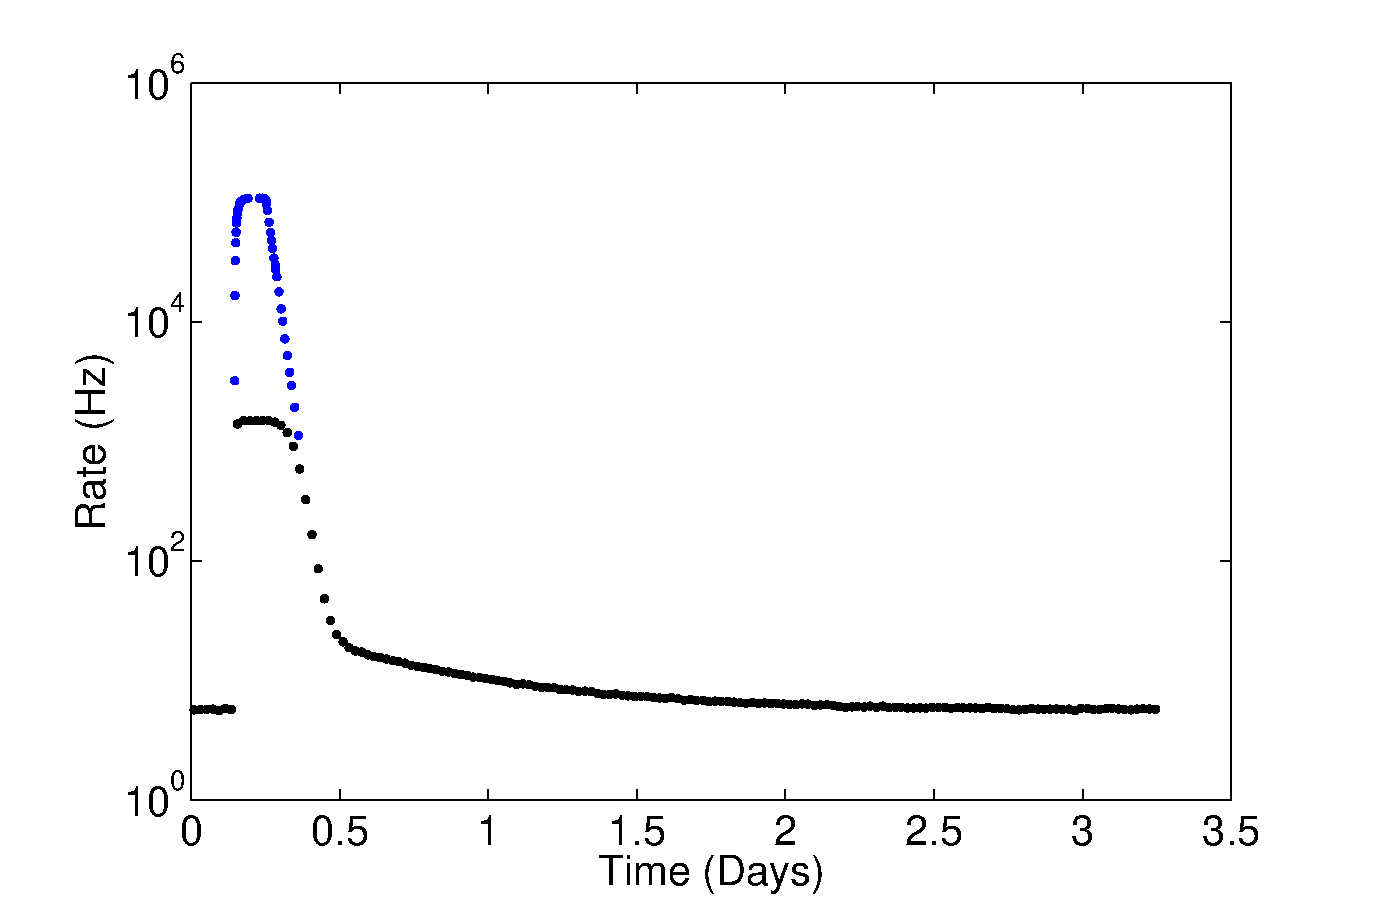
\includegraphics[width=80mm]{fig/TimeHisto_Analog2.eps}
\caption{A time histogram of the event rate during a tritium injection into our small scale detector. The event rate greatly exceeded the limits of our ADC (black data points), so a analog scalar was used to count the true event rate (blue data points). }
\label{fig:Density}
\end{figure}

